\documentclass{beamer}
\usepackage{amsmath}
\usepackage{amssymb}
\usepackage{amsfonts}
\usepackage{bm}

\usepackage{graphicx}
\graphicspath{{./figures/}}
\usepackage{hyperref}
\hypersetup{
  colorlinks=true,
  linkcolor=blue,
  filecolor=magenta,
  urlcolor=blue,
}

\usepackage{tikz}
\usepackage{pgfplots}
\pgfplotsset{compat=1.18}

\usetheme{Boadilla}
\usecolortheme{seahorse}

\title{Bayesian Modeling: A Unified Framework for Probabilistic Reasoning}
\author{Vasilis Gkolemis}
\institute{ATHENA RC | HUA}
\date{June 2025}

\begin{document}

% Automatically insert agenda slide at the start of each section
\AtBeginSection[]{
  \begin{frame}{Program}
    \tableofcontents[currentsection]
  \end{frame}
}

\begin{frame}
  \titlepage
  \vfill
  \footnotesize
  \textcopyright\
  Vasilis Gkolemis, 2025. Licensed under CC BY 4.0.
\end{frame}

\begin{frame}{Contents}
  \tableofcontents
\end{frame}


\begin{frame}{Helping Material}
  \begin{itemize}
    \item \textbf{Primer on Probabilistic Modeling} \url{https://www.inf.ed.ac.uk/teaching/courses/pmr/22-23/assets/notes/probabilistic-modelling-primer.pdf}
  \end{itemize}
\end{frame}


\section{Intro \& Recap}

\begin{frame}{Session 1 – Recap}
  \begin{itemize}
    \item \textbf{What we covered:}
    \begin{itemize}
      \item \textbf{Probabilistic Modeling:}
      Model the world using probabilities
      \item \textbf{Probabilistic Reasoning (Inference):}
      Use knowns to infer unknowns
      \item \textbf{Bayesian Analysis:}
      Modeling and Reasoning with Bayes’ rule.
      \item \textbf{Core Rules of Probability:}
      The sum, product and Bayes’ rule.
      \item \textit{Example: Alzheimer’s diagnostic test.}
    \end{itemize}

    \vspace{0.5cm}
    \item \textbf{What’s still to explore:}
    \begin{itemize}
    \item Our example was simple
      \begin{itemize}
        \item $X$: the test result --- a $1D$ random variable in $\{0, 1\}$
        \item $Y$: the disease status --- a $1D$ random variable in $\{0, 1\}$
      \end{itemize}
    \item Real-world problems are more complex
      \begin{itemize}
      \item Involve high-dimensional random variables
      \item Involve complex relationships between variables
      \end{itemize}
    \item How can we model these complexities?
    \begin{itemize}
      \item Session 2 extended our probabilistic toolbox.
      \item Session 3 will show how to use it in practice.
    \end{itemize}
  \end{itemize}
  \end{itemize}
\end{frame}

\begin{frame}{Session 2 – Recap}
  \begin{itemize}
    \item \textbf{What we covered:}
    \begin{itemize}
      \item \textbf{Multivariate Random Variables and Distributions:}
      \begin{itemize}
        \item PDFs, PMFs and CDFs
        \item Key properties: expectation and variance.
        \item How to sample from these distributions.
        \item Key-distributions: Bernoulli, Normal, Poisson.
      \end{itemize}

      \item We now have powerful tools to model complexity!
    \end{itemize}
    \vspace{0.5cm}
    \item \textbf{What’s still to explore:}
    \begin{itemize}
    \item A glue to connect our probabilistic tools for performing analysis.
    \item A \textit{principled} and \textit{unified} way to:
      \begin{itemize}
        \item Model complex relationships between variables
        \item Infer unknowns from knowns
        \item Make predictions about future observations
      \end{itemize}
   \item The \textbf{Bayesian framework} is (among others) a powerful glue for this.
    \end{itemize}
  \end{itemize}
\end{frame}


\begin{frame}{Session 3 – Overview}
  \begin{itemize}
    \item \textbf{What we’ll explore:}
    \begin{itemize}
      \item The Bayesian Framework with each key components:
      \begin{itemize}
        \item \textbf{Prior Distribution:} Our belief before seeing the data.
        \item \textbf{Likelihood:} How compatible is the observed data is with different parameter values.
        \item \textbf{Posterior Distribution:} Our updated beliefs after observing the data.
        \item \textbf{Predictive Distribution:} Make predictions about new, unseen data.
      \end{itemize}
      \item How to use the Bayesian framework for predictive tasks.
    \end{itemize}
    \vspace{0.5cm}
    \item \textbf{Be confident. You already know important stuff:}
      \begin{itemize}
        \item Session 1:
          \begin{itemize}
            \item Intuition about Bayesian modeling $\rightarrow$ Alzheimer’s test case
            \item Core probability rules: sum, product, and Bayes' rule
            \end{itemize}
          \item Session 2:
            \begin{itemize}
              \item Multivariate random variables and distributions
              \item Key properties: expectation and variance
              \item How to sample from these distributions
            \end{itemize}
    \end{itemize}
  \end{itemize}
\end{frame}

\section{Probabilistic vs statistical vs Bayesian models}

% Slide 13
\begin{frame}{Models}
\begin{itemize}
  \item The term “model” has multiple meanings, see e.g. \url{https://en.wikipedia.org/wiki/Model}
  \item Let's distinguish between three types of models:
  \begin{itemize}
    \item probabilistic model
    \item (parametric) statistical model
    \item Bayesian model
    \end{itemize}
  \item Note: the three types are often confounded, and often just called probabilistic or statistical model, or just “model”.
  \item \href{https://opencourse.inf.ed.ac.uk/sites/default/files/https/opencourse.inf.ed.ac.uk/pmr/2023/probabilistic-modelling-primer.pdf}{Introduction to Probabilistic Modelling} $\rightarrow$ for further reading.

\end{itemize}
\end{frame}

% Slide 14
\begin{frame}{Probabilistic model}
\begin{itemize}
\item From first lecture:
  \begin{quote}
    \vspace{0.4cm}
    A probabilistic model is an abstraction of reality that uses probability theory to quantify the chance of uncertain events.
  \end{quote}
  \vspace{0.2cm}
  \item Example from the first lecture: cognitive impairment test
  \begin{itemize}
    \item Sensitivity of 0.8 and specificity of 0.95 (Scharre, 2010)
    \item Probabilistic model for presence of impairment ($x = 1$) and detection by the test ($y = 1$):
    \begin{itemize}
      \item $P(x = 1) = 0.11$ (prior)
      \item $P(y = 1 \mid x = 1) = 0.8$ (sensitivity)
      \item $P(y = 0 \mid x = 0) = 0.95$ (specificity)
    \end{itemize}
  \end{itemize}
\end{itemize}
\end{frame}

% Slide 15
\begin{frame}{Probabilistic model}
\begin{itemize}
  \item More technically:
  \begin{quote}
    probabilistic model $\equiv$ probability distribution (pmf/pdf).
  \end{quote}
  \item Probabilistic model was written in terms of the probability $P$.
  \item In terms of the pmf it is:
  \begin{itemize}
    \item $p_x(1) = 0.11$
    \item $p_{y \mid x}(1 \mid 1) = 0.8$
    \item $p_{y \mid x}(0 \mid 0) = 0.95$
  \end{itemize}
  \item Commonly written as:
  \begin{itemize}
    \item $p(x = 1) = 0.11$
    \item $p(y = 1 \mid x = 1) = 0.8$
    \item $p(y = 0 \mid x = 0) = 0.95$
  \end{itemize}
  \item where the notation for probability measure $P$ and pmf $p$ are confounded.
\end{itemize}
\end{frame}

% Slide 16
\begin{frame}{Statistical model}
\begin{itemize}
  \item If we substitute the numbers with parameters, we obtain a (parametric) statistical model:
  \begin{itemize}
    \item $p(x = 1) = \theta_1$
    \item $p(y = 1 \mid x = 1) = \theta_2$
    \item $p(y = 0 \mid x = 0) = \theta_3$
  \end{itemize}
  \item For each value of the $\theta_i$, we obtain a different pmf.
  \item Dependency highlighted by writing:
  \begin{itemize}
    \item $p(x = 1; \theta_1) = \theta_1$
    \item $p(y = 1 \mid x = 1; \theta_2) = \theta_2$
    \item $p(y = 0 \mid x = 0; \theta_3) = \theta_3$
  \end{itemize}
\item $p(x, y; \theta)$ where $\theta = (\theta_1, \theta_2, \theta_3)$ is a vector of parameters.
\item or $p(x, y \mid \theta)$, for highlighting that $\theta$ is considered a random variable.

  \item A statistical model corresponds to a set of probabilistic models, here indexed by the parameters $\theta$: $\{p(x; \theta)\}_\theta$
\end{itemize}
\end{frame}

\begin{frame}{What is Bayesian modeling?}

\begin{quote}
A Bayesian model turns a statistical model into a probabilistic one by treating parameters $\theta$ as random variables.
\end{quote}

\vspace{0.5cm}
\textbf{Goal:} Learn what we believe about $\theta$ after seeing data — and use that to make predictions.

\vspace{0.5cm}
\begin{itemize}
\item A Bayesian model is a probabilistic model $p(x, y, \theta)$
\item In supervised settings, we consider $x$ as observed, so we care about $p(y, \theta \mid x)$.
\end{itemize}

\end{frame}


\begin{frame}{Bayesian Modeling in Steps}

\textbf{We don’t know the full joint distribution $p(x, y, \theta)$.}
\begin{itemize}
  \item If we did, every analysis would be trivial.
\end{itemize}

\vspace{0.3cm}
\textbf{What we do have:}
\begin{itemize}
  \item Observed data $\mathcal{D} = \{(x^{(i)}, y^{(i)})\}_{i=1}^N$ — i.i.d. samples from $p(x, y)$
\end{itemize}

\vspace{0.3cm}
\textbf{What we assume:}
\begin{itemize}
  \item $p(y \mid x, \theta)$ — how data is generated given a specific parameter $\theta$
  \item $p(\theta)$ — our beliefs about the parameters before seeing data
\end{itemize}

\vspace{0.3cm}
\textbf{What we want to learn:}
\begin{itemize}
  \item $p(\theta \mid \mathcal{D})$ — what we believe about the parameters after seeing data
  \item The predictive distribution $p(y \mid x, \mathcal{D})$ — predictions that account for parameter uncertainty
  \item Possibly others: e.g. marginal likelihood $p(\mathcal{D})$
\end{itemize}

\end{frame}

\begin{frame}{Bayesian Modeling for Supervised Tasks}

  \begin{itemize}
    \item \textbf{Supervised learning:} We observe a dataset of input–output pairs
    $\mathcal{D} = \{(x^{(i)}, y^{(i)})\}_{i=1}^N$ drawn from an unknown joint distribution $p(x, y)$.

    \item \textbf{Bayesian perspective:} Use this data to learn the relationship $x \mapsto y$ while capturing uncertainty in the model parameters.

    \item \textbf{Hypothesis:}
      \begin{itemize}
        \item (1): assume a parametric family for $p(y \mid x, \theta)$, such as linear regression, neural networks, etc. (Parametric modeling assumption)
        \item (2): assume a prior belief over the parameters $p(\theta)$ (prior assumption)
        \end{itemize}
    \end{itemize}
  \end{frame}

\section{Likelihood}

\begin{frame}{Example: Linear Regression}
  \begin{itemize}
    \item \textbf{Hypothesis:} The outcome depends linearly on some input plus noise.
    \item \textbf{Example:} Predict house price from size.
      \begin{itemize}
        \item $Y$ — house price
        \item $X$ — house size
        \item Model: $Y = wX + b + \epsilon$, with $\epsilon \sim \mathcal{N}(0, \sigma^2)$
      \end{itemize}
    \item $p(Y \mid X; \theta) = \mathcal{N}(Y \mid wX + b, \sigma^2)$
    \item \textbf{Parameters:} $\mathbf{\theta} = (w, b)$ -- 2 variables.
  \end{itemize}
\end{frame}

\begin{frame}{Example: Linear Regression}
  \begin{itemize}
  \item \textbf{Hypothesis:} The outcome depends linearly on some input plus noise.
  \item Generalizes to any number of input features

    \item \textbf{Example:} Predict house price from size, number of rooms, and
      \begin{itemize}
        \item $Y$ — house price
        \item $X = (X_1, X_2, \ldots, X_d)$ — house features (size, number of rooms, etc.)
        \item Model: $Y = wX + b + \epsilon$, with $\epsilon \sim \mathcal{N}(0, \sigma^2)$
        \end{itemize}
    \item $p(Y \mid X; \theta) = \mathcal{N}(Y \mid wX + b, \sigma^2)$
    \item \textbf{Parameters:} $\mathbf{\theta} = (w, b)$: $d+1$ variables.

  \end{itemize}
\end{frame}


\begin{frame}{Example: Non-linear Regression}
  \begin{itemize}
    \item \textbf{Hypothesis:} The relationship between input and output is complex and nonlinear plus noise.
    \item \textbf{Example:} Predict bike rentals from weather data.
      \begin{itemize}
        \item $Y$ — number of bikes rented per hour
        \item $X$ — weather features (temperature, humidity, etc.)
        \item Model $ Y = f_\theta(X) + \epsilon$, with $\epsilon \sim \mathcal{N}(0, \sigma^2)$
          \item $f_\theta(X)$ is a non-linear function parameterized by $\theta$.
          \end{itemize}
        \item $p(Y \mid X; \theta) = \mathcal{N}(Y \mid f_\theta(X), \sigma^2)$
        \item what is $f_\theta(X)$?
          \begin{itemize}
          \item A neural network with weights $\theta$, normally of thousands of variables.
          \item A random forest with decision trees where the structure and parameters are defined by $\theta$, normally of hundreds of variables.
          \end{itemize}
  \end{itemize}
\end{frame}


\begin{frame}{The Flexibility—and Cost—of the Bayesian Framework}

\begin{itemize}
  \item \textbf{Bayesian framework is flexible:}
  We can assume any model for $p(y \mid x, \theta)$.
  \begin{itemize}
    \item Example: $y = f_\theta(x) + \epsilon$, where $\epsilon \sim \mathcal{N}(0, \sigma^2)$
    and $f_\theta(x)$ can be a neural network, random forest, etc.
    \item The output $y$ can follow any distribution — not just Normal:
    skewed, heavy-tailed, discrete (e.g., Poisson, Bernoulli), etc.
  \end{itemize}

\item \textbf{But flexibility comes at a cost}
  \begin{itemize}
    \item the more complex $p(y \mid x, \theta)$:
      \begin{itemize}
      \item Complex $\rightarrow$ a high-dimensional $\theta$.
      \item Complex $\rightarrow$ a complex $f_\theta(x)$
      \end{itemize}
    \item the harder it is to perform inference.
    \end{itemize}
  \end{itemize}

\end{frame}

\begin{frame}
  From $p(y \mid x, \theta)$ to the likelihood function $L(\bm{\theta})$:
  \end{frame}

\begin{frame}
  \frametitle{The likelihood function $L(\bm{\theta})$}

  \begin{itemize}
    \item Measures agreement between $\bm{\theta}$ and the observed data $\mathcal{D}$
    \item Probability that sampling from the model with parameter value $\bm{\theta}$ generates data like $\mathcal{D}$
    \item Exact match for discrete random variables
  \end{itemize}

  \begin{center}
    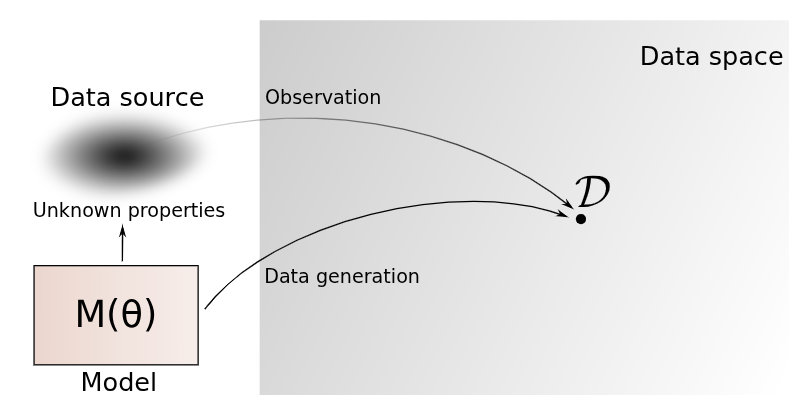
\includegraphics[width=0.7\textwidth]{figures/likelihood_1.png}
  \end{center}
\end{frame}

\begin{frame}
  \frametitle{The likelihood function $L(\bm{\theta})$}

  \begin{itemize}
    \item Measures agreement between $\bm{\theta}$ and the observed data $\mathcal{D}$
    \item Probability that sampling from the model with parameter value $\bm{\theta}$ generates data like $\mathcal{D}$
    \item Small neighbourhood for continuous random variables
  \end{itemize}

  \begin{center}
    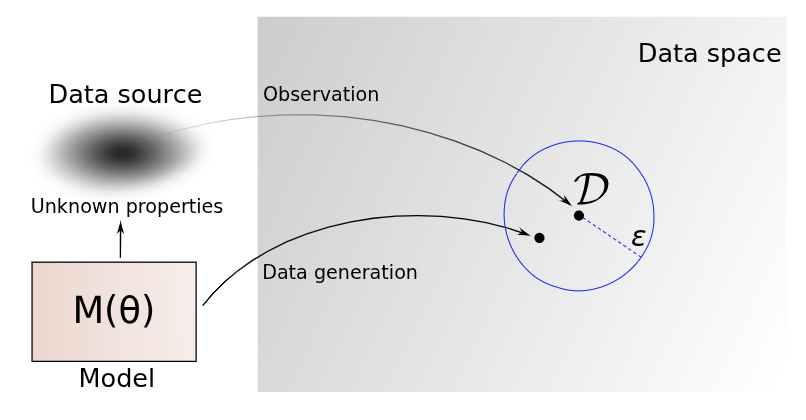
\includegraphics[width=0.7\textwidth]{figures/likelihood_2.png}
  \end{center}
\end{frame}

\begin{frame}
  \frametitle{The likelihood function $L(\bm{\theta})$}

  \begin{itemize}
    \item Probability that the model generates data like $\mathcal{D}$ for parameter value $\bm{\theta}$,
    \[
      L(\bm{\theta}) = p(\mathcal{D}; \bm{\theta})
    \]
    \item[] where $p(\mathcal{D}; \bm{\theta})$ is the parameterised model pdf/pmf.
    \item The likelihood function indicates the likelihood of the parameter values, and not of the data.
    \item For iid data $\bm{x}_1, \dots, \bm{x}_n$
    \[
      L(\bm{\theta}) = p(\mathcal{D}; \bm{\theta}) = p(\bm{x}_1, \dots, \bm{x}_n; \bm{\theta}) = \prod_{i=1}^n p(\bm{x}_i; \bm{\theta})
    \]
    \item Log-likelihood function $\ell(\bm{\theta}) = \log L(\bm{\theta})$. For iid data:
    \[
      \ell(\bm{\theta}) = \sum_{i=1}^n \log p(\bm{x}_i; \bm{\theta})
    \]
  \end{itemize}
\end{frame}

\begin{frame}{Different Perspectives on the Likelihood Function}
 There are different modeling mindsets
  \begin{itemize}
  \item \href{https://christophmolnar.com/books/modeling-mindsets}{Modeling Mindsets} by Christoph Molnar
  \end{itemize}
  \vspace{0.5cm}
  \begin{itemize}
  \item \textbf{Frequentist perspective:}
    \begin{itemize}
    \item Premise: The world is best approached through probability distributions with fixed but unknown parameters.
    \item one set of parameters $\bm{\theta}$ is correct, we just don’t know which one.
    \item Consequence: Find the best parameter values $\bm{\theta}^*$ --- our uncertainty is about whether the parameters are correct.

    \end{itemize}
  \item \textbf{Bayesian perspective:}
    \begin{itemize}
    \item Premise: The world is best approached through probability distributions with probabilistic parameters.
    \item Parameters $\bm{\theta}$ are random variables with a prior distribution $p(\bm{\theta})$.
    \item Consequence: Update the prior parameter distributions using data to obtain the posterior distribution and draw conclusions.
    \end{itemize}
    \end{itemize}
\end{frame}

\begin{frame}{If we were not Bayesians}
  \begin{itemize}
  \item We would use the likelihood function $L(\bm{\theta})$ to find the best parameter values $\bm{\theta}^*$.
    \item Intuition: There is one model that is correct, the one that makes the observed data most probable.
    \item This is called \textbf{maximum likelihood estimation (MLE)}:
      \[
        \bm{\theta}^* = \arg\max_{\bm{\theta}} L(\bm{\theta}) = \arg\max_{\bm{\theta}} p(\mathcal{D}; \bm{\theta})
      \]
    \item MLE does not account for uncertainty in the parameters.
\end{itemize}
  \end{frame}


  \begin{frame}{MLE - Example}
    \begin{itemize}
    \item lets return to the linear gaussian example: \[p(y \mid x; \theta) = \mathcal{N}(y \mid w x + b, \sigma^2)\]
    \item The likelihood function is:
     \[ L(\theta) = p(\mathcal{D}; \theta) = \prod_{i=1}^N p(y^{(i)} \mid x^{(i)}; \theta) \]
   \item The log-likelihood function is:
     \[
       \ell(\theta) = \log L(\theta) = \sum_{i=1}^N \log p(y^{(i)} \mid x^{(i)}; \theta)
     \]
    \item MLE maximizes the likelihood

    \end{itemize}
  \end{frame}

\begin{frame}{MLE - Example}
  \begin{itemize}
    \item MLE finds the parameters $\theta^* = (w, \sigma^2)$ that minimize the negative log-likelihood:
    \[
      \theta^* = \arg\min_{\theta = (w, \sigma^2)} -\ell(\theta)
    \]

    \item For $y_i = wx_i + \varepsilon_i$, with $\varepsilon_i \sim \mathcal{N}(0, \sigma^2)$, the likelihood is:
    \[
      p(y_i \mid x_i, w, \sigma^2) = \frac{1}{\sqrt{2\pi\sigma^2}} \exp\left(-\frac{(y_i - w x_i)^2}{2\sigma^2}\right)
    \]

    \item The negative log-likelihood is:
    \[
      -\ell(w, \sigma^2) = \frac{n}{2} \log(2\pi \sigma^2) + \frac{1}{2\sigma^2} \sum_{i=1}^n (y_i - w x_i)^2
    \]

  \end{itemize}
\end{frame}

\begin{frame}{MLE - Example}
  \begin{itemize}

    \item Minimizing w.r.t. $w$ gives:
    \[
      w^* = \frac{\sum_{i=1}^n x_i y_i}{\sum_{i=1}^n x_i^2}
    \]

    \item Plugging $w^*$ back and minimizing w.r.t. $\sigma^2$ gives:
    \[
      \sigma^{2*} = \frac{1}{n} \sum_{i=1}^n (y_i - w^* x_i)^2
    \]

  \item $w^*$ are the ones that minimize the squared error between the predicted and observed values.
  \item $\sigma^{2*}$ is the variance of the residuals, i.e., the noise in the data.
   \item for new predictions, we can use:
    \[
      p(y \mid x; w^*, \sigma^{2*}) = \mathcal{N}(y \mid w^* x, \sigma^{2*})
    \]
  \end{itemize}
\end{frame}


\begin{frame}{Why MLE is Not Enough}
  \begin{itemize}
    \item \textbf{MLE} finds the parameter $\theta^*$ that makes the data most likely.
    \[
      \theta^* = \arg\max_\theta L(\theta)
    \]
    \item But MLE treats $\theta^*$ as \textit{the truth} — no room for doubt.
    \item \textbf{Problem:} It ignores \textbf{epistemic uncertainty} — our uncertainty about $\theta$.
    \item It only models \textbf{aleatory uncertainty} — randomness in the data.
    \pause
    \item What if:
    \begin{itemize}
      \item We have limited data?
      \item The model is overly complex?
      \item Multiple $\theta$ values explain the data almost equally well?
    \end{itemize}
  \end{itemize}
\end{frame}


\begin{frame}{Why We Are Bayesians: Embracing Uncertainty}
  \begin{itemize}
    \item MLE ranks parameter values via the likelihood $L(\theta)$:
    \[
      L(\theta^*) = \max_\theta L(\theta)
    \]
    \item But many $\theta$ may be almost as plausible!
    \item Especially when:
    \begin{itemize}
      \item data is scarce,
      \item the model is complex,
      \item or the model is mis-specified.
    \end{itemize}
    \vspace{0.5em}
    \item \textbf{Bayesian modeling} treats $\theta$ as a \textit{random variable}, not a fixed value.
    \item We don’t commit to one model — we reason over a \textbf{distribution of plausible models}.
    \item This gives us a posterior distribution:
    \[
      p(\theta \mid \mathcal{D})
    \]
    capturing our full uncertainty given the data.
  \end{itemize}
\end{frame}

\section{Inference}

\begin{frame}{Prior and Posterior}
  \begin{itemize}
    \item \textbf{Prior distribution} $p(\theta)$: Our beliefs about the parameters before seeing data.
    \item \textbf{Posterior distribution} $p(\theta \mid \mathcal{D})$: Our updated beliefs after observing data $\mathcal{D}$.
    \item The posterior is computed using Bayes' rule:
    \[
      p(\theta \mid \mathcal{D}) = \frac{p(\mathcal{D} \mid \theta) p(\theta)}{p(\mathcal{D})} = \frac{L(\theta) p(\theta)}{p(\mathcal{D})}
    \]
    where:
    \begin{itemize}
      \item $p(\mathcal{D} \mid \theta)$ is the likelihood function.
      \item $p(\mathcal{D})$ is the marginal likelihood, a normalizing constant.
      \end{itemize}
    \item we often write $p(\theta \mid \mathcal{D}) \propto p(\mathcal{D} \mid \theta) p(\theta)$
  \end{itemize}
\end{frame}

\begin{frame}{Predictive Posterior}
  \begin{itemize}
    \item \textbf{Predictive posterior} $p(y \mid x, \mathcal{D})$: Our predictions about new data $y$ given input $x$ and observed data $\mathcal{D}$.
    \item It accounts for uncertainty in the parameters $\theta$:
    \[
      p(y \mid x, \mathcal{D}) = \int p(y \mid x, \theta) p(\theta \mid \mathcal{D}) d\theta
    \]
    where:
    \begin{itemize}
      \item $p(y \mid x, \theta)$ is the model likelihood for a specific parameter $\theta$.
      \item $p(\theta \mid \mathcal{D})$ is the posterior distribution of the parameters.
    \end{itemize}
  \item This integral averages over all plausible parameter values, weighted by their posterior probability.
  \item Normally, it is impossible to compute analytically, so we use approximations and sampling methods.
    \end{itemize}
  \end{frame}

  \begin{frame}{Predictive Posterior using samples}
  \begin{itemize}
  \item If we have samples from the posterior:
    \[ \theta^m \sim p(\theta \mid \mathcal{D}) \text{ for } m = 1, \ldots, M \]

  \item
    we can make predictions by sampling from the predictive posterior:
    \[
      y^m \sim p(y \mid x, \theta^m) \text{ for } m = 1, \ldots, M
    \]
  \item This gives us a set of predictions $\{y^m\}_{m=1}^M$ with:
    \begin{itemize}
      \item Expectation:
        \[
          \hat{y} = \frac{1}{M} \sum_{m=1}^M y^m
        \]
      \item Variance:
        \[
          \hat{\sigma}^2 = \frac{1}{M} \sum_{m=1}^M (y^m - \hat{y})^2
        \]
    \end{itemize}
  \item This approach captures uncertainty in the predictions by averaging over all plausible parameter values.
    \end{itemize}
\end{frame}

\begin{frame}{Conclusion}
  \begin{itemize}
    \item We have seen how to use the Bayesian framework for probabilistic modeling.
    \item We have learned how to:
      \begin{itemize}
        \item Define a prior distribution over parameters.
        \item Compute the likelihood function from observed data.
        \item Update our beliefs using Bayes' rule to obtain the posterior distribution.
        \item Make predictions using the predictive posterior.
      \end{itemize}
    \item The Bayesian framework allows us to reason about uncertainty in a principled way.
    \item Next, we will explore practical applications and tools for Bayesian modeling.
    \end{itemize}
\end{frame}

\end{document}
